\documentclass{article}
\usepackage[T2A]{fontenc}
\usepackage{epigraph}
\usepackage[english, russian]{babel} % языковой пакет
\usepackage{amsmath,amsfonts,amssymb} %математика
\usepackage{mathtools}
\usepackage[oglav,spisok,boldsect,eqwhole,figwhole,hyperref,hyperprint,remarks,greekit]{../../style/fn2kursstyle}
\usepackage[utf8]{inputenc}
\usepackage[]{tkz-euclide}
\usepackage{algpseudocode}
\usepackage{pgfplots}
\usepackage{tikz-3dplot}
\usepackage[oglav,spisok,boldsect,eqwhole,figwhole,hyperref,hyperprint,remarks,greekit]{./style/fn2kursstyle}
\usepackage{multirow}
\usepackage{supertabular}
\usepackage{multicol}
\usepackage{tikz}
\usepackage{pgfplots}
\usepackage{float}
\usepackage{graphicx}
\pgfplotsset{compat=1.9}
\usepackage[svgnames]{pstricks}
\usepackage{pst-solides3d} 
\usepackage{multirow}
\usepackage{hhline}
\usepackage{slashbox}
\usepackage{pdflscape}
\usepackage{array} 
\graphicspath{{../../style/}}

  



\newcommand{\cond}{\mathop{\mathrm{cond}}\nolimits}
\newcommand{\rank}{\mathop{\mathrm{rank}}\nolimits}
% Переопределение команды \vec, чтобы векторы печатались полужирным курсивом
\renewcommand{\vec}[1]{\text{\mathversion{bold}${#1}$}}%{\bi{#1}}
\newcommand\thh[1]{\text{\mathversion{bold}${#1}$}}
%Переопределение команды нумерации перечней: точки заменяются на скобки
\renewcommand{\labelenumi}{\theenumi)}
\newtheorem{theorem}{Теорема}
\newtheorem{define}{Определение}
\tdplotsetmaincoords{60}{115}
\pgfplotsset{compat=newest}

\title{Итерационные методы решения систем
линейных алгебраических уравнений}
\author{Н.\,О.~Акиньшин}
\group{ФН2-51Б}
\date{2024}
\supervisor{А.\,С.~Джагарян}



\begin{document}
    \maketitle
    \newpage
    \tableofcontents
    \newpage

    \section{Контрольные вопросы}
    \begin{enumerate}
        \item Почему условие $\|C\| < 1$ гарантирует сходимость итерационных методов?
        \newline
        {\bfseries Ответ.}
        Любой одношаговый итерационный метод можно записать в виде 
        \begin{equation*}
            B_{k+1}\frac{x^{k+1} - x^k}{\tau_{k+1}} + A x^k = b, \ k = 0, 1, 2,\ldots
        \end{equation*}
        Из этого вида можно прийти к следующему:
        \begin{equation}
            x^{k+1} = Cx^k + y
            \label{special form iter method}
        \end{equation}
        Подставив истинное решение $x$ в~\eqref{special form iter method},
        получим 
        \begin{equation*}
            x \equiv  Cx + y 
        \end{equation*}
        Тогда, вычитая из~\eqref{special form iter method},
        \begin{equation*}
            x^{k+1} - x = C(x^{k} - x)
        \end{equation*}
        Переходя к выражению с нормами
        \begin{equation*}
            \|x^{k+1} - x\| = \|C(x^{k} - x)\| \leqslant
           \|C\| \|x^{k} - x\| \leqslant \ldots \leqslant \|C\|^{k}\|x_0 - x\|
        \end{equation*}
        Если $\|C\| < 1$, то последовательность сходится $\{x^k\}_{k=1}^\infty$ сходится к $x$ для 
        любого $x_0$.

        
        \item Каким следует выбирать итерационный параметр $\tau$ в методе 
        простой итерации для увеличения скорости сходимости?
        Как выбрать начальное приближение $x_0$?
        \newline
        {\bfseries Ответ.}
        Пусть $x$-истинное решение системы $Ax=f$. Метод простой итерации можно представить в виде $\frac{x^{k+1}-x^k}{\tau}+Ax^k=f$, где $x^k$--koе приближение истинного решения. Введем обозначение $z^k=x^k-x$--погрешность. Тогда метод простой итерации можно переписать $\frac{z^{k+1}-z^k}{\tau}+Az^k=0$. Отсюда $z^{k+1}=(E + \tau A) z^k$. Перейдем к норме
	\[
	||z^{k+1}||\le||(E + \tau A)|| \cdot ||z^k||\le ||(E + \tau A)||^{k+1} \cdot ||z^0|| =||(E + \tau A)||^{k+1} \cdot ||x^0-x||
	\]
	Из данного соотношения можно сделать вывод, что параметр $\tau$ нужно выбрать так чтобы норма матрицы $(E+\tau A)$ была как можно меньше, а начальное приближение выбрать как можно ближе к истинному решению.

        \item На примере системы из двух уравнений с двумя неизвестными
        дайте геометрическую интерпретацию метода метода
        Якоби, метода Зейделя, метода релаксации.
        \newline
        {\bfseries Ответ.}
        Рассмотрим метод Якоби.
        \begin{equation}
            \begin{dcases}
                a_{11}x_1^{k+1} + a_{12}x_2^k = b_1, \\
                a_{21}x_1^{k} + a_{22}x_2^{k+1} = b_2,
            \end{dcases}
            \label{system_jacoby}
        \end{equation}
        Пусть $l_1: a_{11}x_1^{k+1} + a_{12}x_2^k = b_1$, и 
        $l_2: a_{21}x_1^{k} + a_{22}x_2^{k+1} = b_2$ -- прямые, задаваемые уравнениями системы.
        Точка их пересечения и есть истинное решение системы~\eqref{system_jacoby}. 
        На рис.~\ref{jacoby_graph} видно, что с каждой итерацией точка $x^k = (x_1^k, x_2^k)$ 
        сходится к истинному решению $x$, причем каждая точка $x^k$ лежит внутри области, ограниченных прямыми.
        Причем ни одна из итеративных точек не лежит на прямых.
        \begin{figure}[H]
            \center
            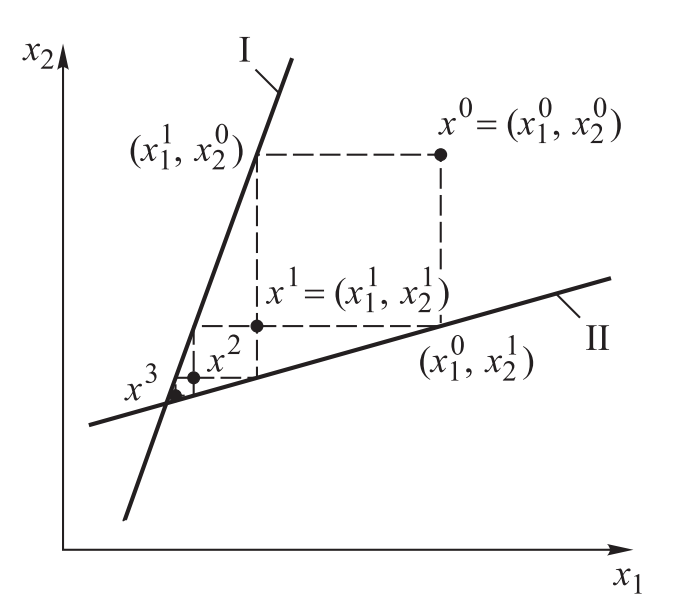
\includegraphics[width=0.5\textwidth]{jacoby_graph.png}
            \caption{Графический смысл метода Якоби}
            \label{jacoby_graph}
        \end{figure}
        Рассмотрим метод Зейделя.
        \begin{equation}
            \begin{dcases}
                a_{11}x_1^{k+1} + a_{12}x_2^k = b_1, \\
                a_{21}x_1^{k+1} + a_{22}x_2^{k+1} = b_2,
            \end{dcases}
            \label{system_seidel}
        \end{equation}
        Аналогично, принимая за прямые $l_1 = a_{11}x_1^{k+1} + a_{12}x_2^k = b_1$ и 
        $l_2 = a_{21}x_1^{k+1} + a_{22}x_2^{k+1} = b_2$ за прямые. Изобразим эти прямые на 
        рис.~\ref{seidel_graph}. Из рис.~\ref{seidel_graph} видно, что все точки лежат на прямых.
        \begin{figure}[H]
            \center
            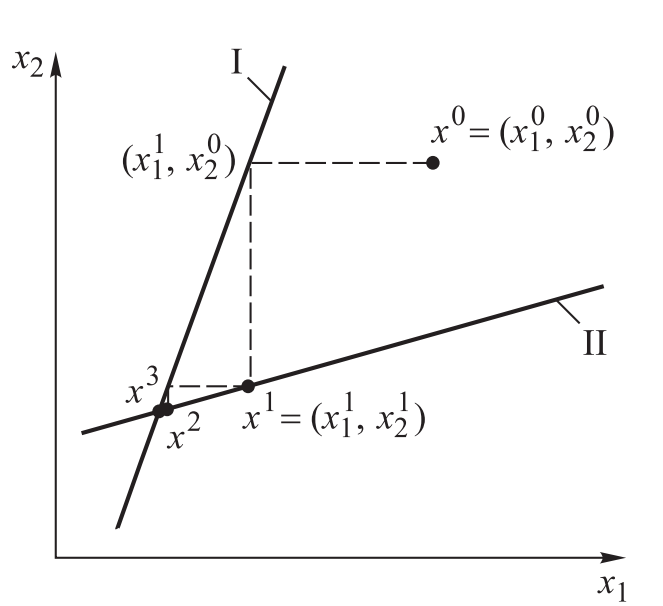
\includegraphics[width=0.5\textwidth]{seidel_graph.png}
            \caption{Графический смысл метода Зейделя}
            \label{seidel_graph}
        \end{figure}

        Рассмотрим метод релаксации. 
        \begin{equation}
            \begin{dcases}
                a_{11} (x_1^{k+1} - x_1^k) = \omega (-a_{11}x_1^k - a_{12}x_2^k +f_1), \\ 
                a_{22} (x_2^{k+1} - x_2^k) = \omega (-a_{21}x_1^k - a_{22}x_2^k +f_2)
            \end{dcases}
        \end{equation}
        Пусть $\boldsymbol{l_1} = (a_{11}, -a_{12})$ -- вектор нормали первой прямой, тогда 
        величина 
        \begin{equation*}
        |\omega (-a_{11}x_1^k - a_{12}x_2^k +f_1)| = \omega d_1 \|\boldsymbol{l_1}\|,
        \end{equation*}
        где $d_1$ -- расстояние от $(x_1^k, x_2^k)$ до первой прямой.
        При этом направление смещения вдоль оси
        абсцисс определяется тем, в положительной или отрицательной
        полуплоскости относительно прямой I расположена точка $(x_1^k, x_2^k)$.
        Заметим, что 
        \begin{equation*}
            |x_1^{k+1} - x_1^k| = \omega \dfrac{d_1}{|a_{11} / \|\boldsymbol{l_1}\||} = 
            \omega \dfrac{d_1}{|\cos \beta_1|},
        \end{equation*}
        где $\beta_1$ -- угол между первой прямой и осью координат.

        \begin{figure}[H]
            \center
            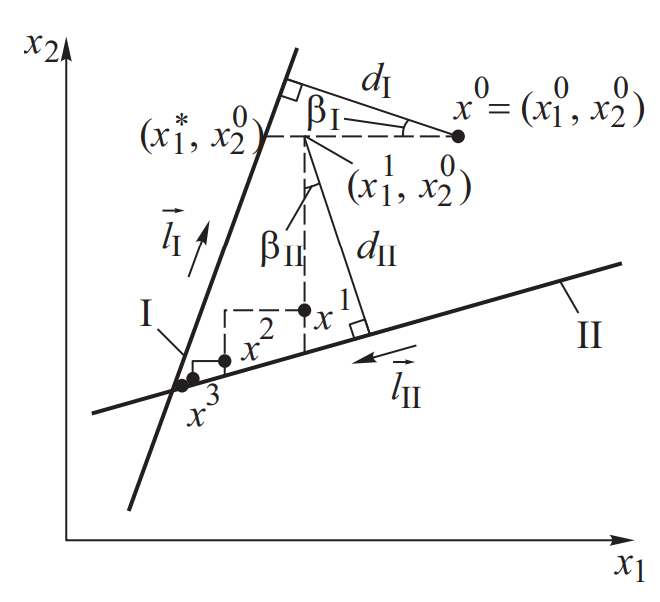
\includegraphics[width=0.5\textwidth]{lower_relaxation.png}
            \caption{Графический смысл метода релаксации при $\omega < 1$}
            \label{lower_relax_graph}
        \end{figure}

        \begin{figure}[H]
            \center
            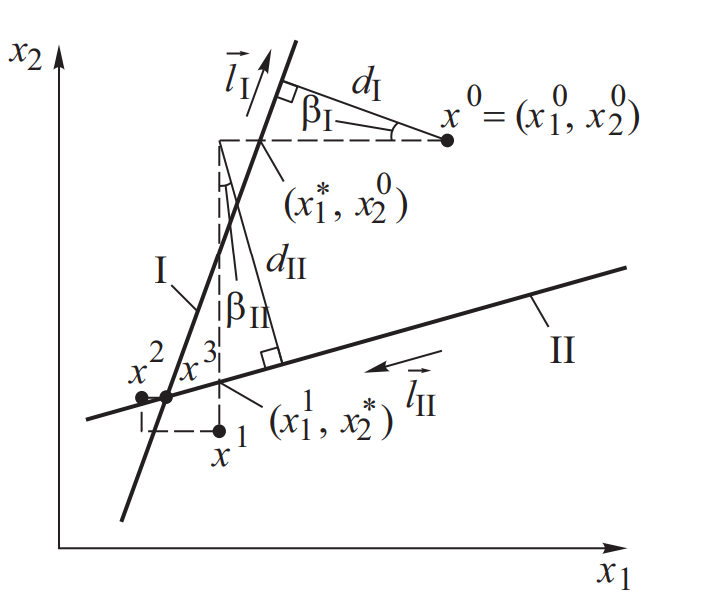
\includegraphics[width=0.5\textwidth]{upper_relaxation.png}
            \caption{Графический смысл метода релаксации при $\omega > 1$}
            \label{upper_relax_graph}
        \end{figure}

        \item При каких условиях сходятся метод простой итерации,
        метод Якоби, метод Зейделя и метод релаксации? Какую
        матрицу называют положительно определенной?
        \newline
        {\bfseries Ответ.}
        \textbf{Определение} Матрица $A$ называется положительно определенной $A>0$, если $\forall x \, (Ax, x) > 0 $.
	
	
	\noindent Рассмотрим теорему о сходимости стационарного итерационного метода.
	
	\textbf{Теорема} Пусть $A--$ симметричная положительно определенная матрица, $\tau > 0$ и выполнено неравенство 
	\[
	B-0.5\tau A
	\]
	Тогда стационарный итерационный метод 
	\[
	B\frac{x^{k+1}-x^k}{\tau} + Ax^k = f
	\]
	сходится при любом начальном приближении $x^0$.
	
	
	\textbf{Доказательство} Пусть $x^k=x^k-x$--погрешность k--й итерации. Поскольку $f=Ax$, то 
	\[
	B\frac{z^{k+1}-z^k}{\tau} + Az^k = 0
	\]
	Необходимо показать,что норма погрешности стремится к нулю при $k \rightarrow \infty$. Проведем преобразования:
	\[
	z^{k+1}=(E-\tau B^{-1}A)z^k
	\]
	\[
	Az^{k+1}=(A-\tau AB^{-1}A)z^k
	\]
	\[
	(Az^{k+1},z^{k+1})= ((A-\tau AB^{-1}A)z^k, (E-\tau B^{-1}A)z^k)=
	\]
	\[
	(Az^k,z^k)-\tau (Az^k,B^{-1}Az^k) - \tau (AB^{-1}Az^k,z^k) + \tau^2(AB^{-1}Az^k,B^{-1}Az^k).
	\]
	В силу симметрии A имеем 
	\[
	(AB^{-1}Az^k,z^k) = (B^{-1}Az^k, Az^k)
	\]
	Следовательно,
	\[
	J_{k+1}=(Az^{k+1},z^{k+1}) = J_{k} - 2 \tau ((B-0.5 \tau A)B^{-1}Az^k,B^{-1}Az^k) + \tau^2(AB^{-1}Az^k,B^{-1}Az^k)
	\]
	\[
	J_{k+1}=J_k- 2 \tau ((B-0.5 \tau A)B^{-1}Az^k,B^{-1}Az^k)
	\]
	
	Если $B-0.5\tau A>0$, то $J_{k+1}\le J_{k}, J_{k} \ge 0$, так как $A>0$. Отсюда заключаем, что последовательность $J_k$ монотонно не возрастает и ограничена нулем снизу. Поэтому существует предел последовательности: $\lim \limits_{k \rightarrow \infty} J_k = J$. Положительная определенность матрицы $B-0.5\tau A$ означает, что верна оценка 
	\[
	((B-0.5\tau A)y,y) \ge \delta ||y||^2
	\]
	Следовательно, 
	\[
	J_{k+1}-J_k+2\tau \delta ||B^{-1}Az^k||^2 \le 0
	\]
	откуда при $k \rightarrow \infty$ получим $\lim\limits_{k \rightarrow \infty } ||B^{-1}Az^k||^2=0$. Введем обозначение $w_k=B^{-1}Az^k$, тогда $z^k=A^{-1}B w_k$. Отсюда $||z^k|| \le ||A^{-1}B|| \cdot ||w_k||$ и $\lim \limits_{k \rightarrow \infty}||z^k||=0$.
	
	\textbf{Следствие} Пусть A--симметричная положительно определенная матрица с диагональным преобладанием,т.е. 
	\[
		a_{ii} > \sum_{j=1,j \neq i}^{n} |a_{ij}|, \, i=1 \ldots n.
	\]
	Тогда метод Якоби сходится.
	
	\textbf{Доказательство} Условие сходимости в данном случае имеет вид $D-0.5A \Rightarrow A<2D$. Рассмотрим положительно определенную форму
	\[
	(Ax,x)= \sum_{i,j}a_{ij}x_i x_j.
	\] 
	Для нее имеем оценку 
	\[
	(Ax,x) \le 0.5 \sum_{i,j} |a_{ij}| x_i^2 + 0.5 \sum_{i,j} |a_{ij}| x_j^2=0.5 \sum_{i,j} |a_{ij}| x_i^2 + 0.5 \sum_{i,j} |a_{ji}| x_i^2 = \sum_{i,j}|a_{ij}| x_i^2
	\]
	Последнее равенство верно в силу симметричности матрицы A. Отсюда 
	\[
	(Ax,x) \le \sum_{i,j}|a_{ij}| x_i^2 = \sum_{i=1}^{n}x_i^2(|a_{ii}|+\sum_{j=1, j\neq i}^{n}|a_{ij}|)
	\]
	Однако вследствие положительной определенности матрицы $a_{ii}>0, \, i=1 \ldots n$. Используя условие диагонального преобладания, имеем 
	
	\[
	(Ax,x) < \sum_{i=1}^{n} x_i^2(a_{ii}+a_{ii})=2(Dx,x)
	\]
	
		
	\textbf{Следствие} Пусть A--симметричная положительно определенная матрица. Тогда метод релаксации сходится при $0<w<2$. В частности, сходится метод Зейделя $(w=1)$
 
	\textbf{Доказательство} Для данного метода $B=D+wA_1; \tau =w; A=A_1+D+A_2$. В случае симметричной матрицы имеем $A_1^*=A_2$. Нужно показать, что
	\[
	(D+wA_1)-0.5w(A_1+D+A_2)>0.
	\]
	При $0<w<2$
	\[
	((B-0.5\tau A)x,x) = (1-0.5w)(Dx,x)+0.5w(A_1x,x) -0.5w(A_2x,x)=(1-0.5w)(Dx,x) >0
	\]
	Так как D -- положительная определенная матрица.
	
	\textbf{Следствие} Метод простой итерации сходится при $\tau < 2/\lambda_{max}$, где $\lambda_{max}$ -- максимальное собственное значение симметричной положительно определенной матрицы A.
	
	\textbf{Доказательство} Условие $B-0.5 \tau A >0$ в данном случае есть $E-0.5 \tau A >0$, что эквивалентно условию положительности минимального собственного значения матрицы $E-0.5 \tau A$, т.е. $1-0.5 \tau \lambda_{max} >0$

        \item Выпишите матрицу $C$ для методов Зейделя и релаксации.
        \newline
        {\bfseries Ответ.} 
        Рассмотрим метод Зейделя.
        Будем считать, что $A = L + D + U$, где $L$ -- нижнетреугольная матрица, $D$ -- 
        диагональная матрица, $U$ -- верхнетреугольная матрица.
        Тогда метод Зейделя можно представить в каноническом виде: 
        \begin{equation*}
            (D + L)(x^{k+1} -x^k) + Ax^k = f
        \end{equation*}
        Из этого вида получаем:
        \begin{equation*}
            C = E - (D+L)^{-1}A
        \end{equation*}

        Рассмотрим метод релаксации.
        Метод релаксации можно представить в каноническом виде: 
        \begin{equation*}
            (D + \omega L)\frac{x^{k+1} -x^k}{\omega} + Ax^k = f
        \end{equation*}
        Тогда 
        \begin{equation*}
            C = E - \omega(D+\omega L)^{-1}A
        \end{equation*}
        \item Почему в общем случае для остановки итерационного
        процесса нельзя использовать критерий $\|x^k - x^{k+1}\| < \varepsilon$?
        \newline
        {\bfseries Ответ.}
        Потому, что $||x^{k}-x^{k-1}||$ может быть меньше $\epsilon$, однако $x^k$ будет плохо приближать истинное решение т.е. для любого $\epsilon, \delta$ в общем случае можно подобрать такие уравнения, чтобы  $||x^{k}-x^{k-1}|| < \epsilon$, но $||x^{k}-x|| > \delta$. Рассмотрим на примере системы из 2ух уравнений. В таком случаи уравнения будут представлять прямые, а решение системы пересечение прямых. Чтобы сделать маленькую разницу между предыдущим и текущим приближением нужно задать прямые достаточно параллельно т.е. острый угол между прямыми сделать достаточно маленьким.

        
        \item Какие еще критерии окончания итерационного процесса
        Вы можете предложить?
        \newline
        {\bfseries Ответ.}

        Рассмотрим критерий останова $\|x^{k+1} - x^k\| < \varepsilon$. Его достоинством
        можно считать простоту вычисления, однако он обладает существенным недостатком. Если 
        алгоритм уменьшает скорость схождения, но при этом не сходится к истинному решению, то данный 
        критерий вынудит алгоритм остановиться, а также не отражает связи между истинным решением и полученным: 
        \begin{equation*}
            \|x^{k+1} - x^k \| = \|x^{k+1} - x + x - x^k\| \leqslant \|x^{k+1} - x\| + \|x^k - x\| \not \leqslant \varepsilon   
        \end{equation*}

        Рассмотрим критерий останова 
        $\dfrac{\|x^{k+1} - x^k\| }{\|x^k\|+ \varepsilon_0} < \varepsilon$.
        Его достоинством по сравнению с предыдущем критерием является то, что 
        он вычисляет разность между решениями относительно предыдущего решения, то есть 
        он может заставить алгоритм остановиться только тогда, когда относительная скорость 
        схождения будет достаточно малой, в отличие от абсолютной, как это указано в предыдущем критерии.
        Недостатком можно считать наличие двух параметров $\varepsilon_0, \ \varepsilon$.

        Рассмотрим критерий останова $\|Ax^k - f \|< \varepsilon$. Среди достоинств можно отметить, что 
        он не реагирует на скорость схождения алгоритма. Однако он может оказаться неприемлимым, когда 
        норма матрицы $A$ достаточно мала.   

        Рассмотрим критерий останова $\dfrac{\|r^k\|}{\|r^0\|} < \varepsilon$. Достоинством можно считать 
        не такая сильная зависимость от нормы матрицы $A$. Недостатком является, что если мы выберем $x_0$ 
        достаточно близко к истинному решению $x$, то невязка $r_0$ будет близко к 
        0, и при вычислении критерия будет большая погрешность. 

        Рассмотрим критерий останова $\dfrac{\|C\|}{1-\|C\|} \|x^{k+1} - x^k\| < \varepsilon$.
        
        Заметим, что 
        \begin{equation*}
            \|x^{k+1} - x\| = \|C(x^k+1 - x^k) + C(x^k - x)\| \leqslant
            \|C\| \|x^{k+1} - x^k\| + \| C\| \|x^k - x\|
        \end{equation*}
        Тогда
        \begin{equation*}
            \|z^k\| \leqslant \dfrac{\|C\|}{1-\|C\|} \|x^{k+1} - x^k\| < \varepsilon
        \end{equation*}
        Благодаря данному критерию можно ограничивать погрешность между истинным и полученным решением. 
        Недостатком является необходимость вычислять матрицу $C$, хранить её и вычислять норму. 


    \end{enumerate}

    \section{Дополнительные вопросы}
    \begin{enumerate}
        \item Сформулировать теорему о сжимающем отображении
        
        {\bfseries Ответ. }
    {\bfseries Определение. } $(X, \rho)$ называют метрическим пространством, если задана функция 
    $\rho: X \rightarrow \mathbb{R}$, которая удовлетворяет следующим свойствам: 
    \begin{enumerate}
        \item $\forall x, y\,  \in\, X: \  \rho(x,y) \geqslant 0$, причем $\rho(x,y) = 0 \Leftrightarrow x = y = 0$;
        \item $\forall x, y \, \in \, X \  \rho(x,y) = \rho(y,x)$;
        \item $\forall x, y, z \, \in \, X \ \rho(x,z) \leqslant \rho(x,y) + \rho(y,z)$;
    \end{enumerate}
    
    {\bfseries Определение. } Метрическое пространство $(X, \rho)$ называется полным, если в нем сходится любая 
    фундаментальная последовательность.

    Пример полного м.п.: 
    Пусть $X = \mathbb{R}$ и для любых чисел $x, y \in X \rho(x,y) = |x-y|$. Тогда по критерию
    Коши, числовая последовательность сходится $\Leftrightarrow$ она является фундаменальной.
    
    Пример неполного м.п.: 
    Пусть $Y = \mathbb{Q}$ и для любых $x, y \in Y \rho (x,y) = |x-y| $


        {\bfseries Определение. } Пусть $(X, \rho)$ - метрическое пространство. Отображение 
        $g : X \rightarrow X$ называется сжимающим $\Leftrightarrow \exists \, \alpha \in (0,\, 1): \forall x, \, y \in X: \rho(g(x),\,g(y)) \leqslant \alpha \,\rho(x,y)$ 
        


        {\bfseries Теорема. } Любое сжимающее отображение $g: X \rightarrow X$ в полном 
        метрическом пространстве $(X, \rho)$ имеет, и притом только одну неподвижную точку, то есть 
        $\exists!\, x\in X: g(x) = x$ 
        {\bfseries Доказательство.} Выберем произвольную точку $x_0 \in X$. Рассмотрим последовательность
        $\{x_n\}_{n=1}^\infty$:
        \begin{align*}
            x_1 &= g(x_0), & x_2 &= (x_1), & \ldots& & x_n &= g(x_{n-1}), & \ldots &
        \end{align*}
        Докажем, что $\{x_n\}_{n=1}^\infty$ фундаментальна в $X$:
        
        Выберем любые $n \in \mathbb{N} $ и $m > n$, тогда по определению сжимающего отображения: 
        \begin{gather*}
            \rho(x_n, x_m) = \rho(g(x_{n-1}), g(x_{m-1})) \leqslant \\
            \leqslant \alpha \rho(x_{n-1}, x_{m-1}) = \rho(g(x_{n-2}), g(x_{m-2})) \leqslant \\
            \leqslant \alpha^2 \rho(x_{n-2}, x_{m-2}) \leqslant \ldots \leqslant \alpha^n \rho(x_0, x_{m-n})\leqslant \\
            \leqslant \alpha^n (\rho(x_0, x_1), + \rho(x_1, x_2) + \ldots + \rho(x_{m-n-1},x_{m-n})) \leqslant \\
            \leqslant \alpha^n \rho(x_0, x_1) (1 + \alpha + \ldots + \alpha^{m-n-1}) < \frac{\alpha^n}{1-\alpha} \rho(x_0, x_1),
        \end{gather*}
        где $\alpha \in (0,\, 1)$. 

        Поскольку $\lim\limits_{n \to \infty} \alpha^n = 0$, то для любого числа 
        $\varepsilon > 0$ найдется такое натуральное число $N$, что для всяких 
        $n > N$ и $m >n$ верно
        \begin{equation*}
            \rho(x_n, x_m) < \frac{\alpha^n}{1-\alpha} \rho(x_0, x_1) < \varepsilon
        \end{equation*}
        Тогда, исходя из данного неравенства, $\{x_n\}_{n=1}^\infty$ является фундаменальной.
        В силу полноты $(X, \rho)$, то существует предел $x\in X$
        последовательности $\{x_n\}_{n=1}^\infty$
        Докажем, что это неподвижная точка, т.е. $g(x) = x$. 
        \begin{gather*}
            0 \leqslant \rho(x, g(x)) \leqslant \rho(x, x_n) + \rho(x_n, g(x)) = \\ 
            = \rho(x, x_n) + \rho(g(x_{n-1}), g(x)) \leqslant \rho(x, x_n) + \alpha \rho(x_{n-1}, x) \to 0 \text{ при } {n\to \infty}
        \end{gather*}
        Следовательно, $\rho(x, g(x)) = 0$, и $g(x) = x$.

        Докажем, что такая точка единственна. Пусть существует еще одна неподвижная точка 
        $y \in X, y \neq x$ и $g(y) = y$. Тогда справедливо
        \begin{equation*}
            \rho(x,y) = \rho(g(x), g(y)) \leqslant \alpha \rho(x,y) < \rho(x,y),
        \end{equation*}
        чего не может быть, следовательн $x = y$. {\bfseries Доказано.}
        \item Чему равно значение параметра $\tau$, при котором норма матрицы $C$ минимальна?
        
        {\bfseries Ответ. }
        1)Общий случай. Любой итерационный алгоритм можно представить в виде.
	\[
	B_{k+1} \frac{x^{k+1}-x^k}{\tau ^k}+Ax^k=f
	\]
	Приведем к виду $x^{k+1} = Cx^k +y$. Получим
	\[
	x^{k+1} = (E - \tau_k B_{k+1}^{-1}A)x^k + \tau_k B_{k+1}^{-1}f
	\]
	Тогда $C = E - \tau_k B_{k+1}^{-1}A, y =\tau_k B_{k+1}^{-1}f$. Тогда норму матрицы C можно найти $|C|| = ||E - \tau_k B_{k+1}^{-1}A||$. Из соотношения можно сделать вывод, что для того чтобы $||C||$ была минимальна нужно выбирать параметры $\tau_k$ так, чтобы $||E - \tau_k B_{k+1}^{-1}A||$ была минимальной.
	
	2) Пусть имеем положительно определенные, самосопряженные матрицы A, B такие, что выполняется неравенство $\gamma_1 B\le A \le \gamma_2 B$. Будем рассматривать стационарный итерационный алгоритм т.е.
	\[
	B\frac{x^{k+1}-x^k}{\tau}+Ax^k=f
	\]
	Аналогично 1 можно показать $C = E - \tau B^{-1}A, ||C|| = ||E - \tau B^{-1}A||$. Данное неравенство можно переписать в виде  $\gamma_1 \le B^{-1}A \le \gamma_2$, что равносильно неравенству $\gamma_1 (x,x) \le (B^{-1}Ax,x) \le \gamma_2 (x,x)$. Домножим на -$\tau$ и прибавим $(x,x)$ Получим следующее. $(x,x)-\tau \gamma_2 (x,x) \le (x,x) + (-\tau B^{-1}Ax,x) \le (x,x)-\tau \gamma_1 (x,x)$. В итог получим следующее неравенство.
	\[
	(1-\tau \gamma_2) (x,x) \le (E-\tau B^{-1}Ax,x) \le (1-\tau \gamma_1) (x,x)
	\]
	Что равносильно
	\[
	(1-\tau \gamma_2) \le E-\tau B^{-1}A \le (1-\tau \gamma_1), C =E-\tau B^{-1}A 
	\]
	Поскольку операторы A, B самосопряженные, то $E-\tau B^{-1}A$, также самосопряжен. Тогда Неравенство позволяет оценить спектр оператора $C=E-\tau B^{-1} \le max(|1-\tau \gamma_2|, |1-\tau \gamma_1|) = N(\tau)$ т.к норма самосопряженного оператора есть максимальное по модулю собственное значение. Если минимизировать выражение $N(\tau)$, то $||C||$ будет минимальна. Таким образом нужно найти величину $\min \limits _{\tau} N(\tau) = \min \limits_{\tau} \max(|1-\tau \gamma_2|, |1-\tau \gamma_1|)$. Для этого изобразим в осях $N vs \tau$.
	
	% Картинка из учебника
	\begin{figure}[H]
        \center
        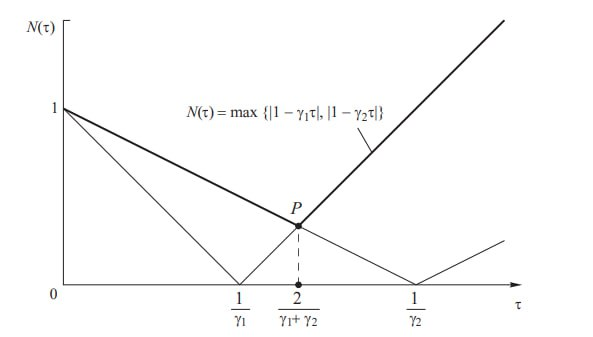
\includegraphics[width=0.7\textwidth]{vopros2.jpg}
        \caption{Графическая зависимость $N(\tau)$}
        \label{vopros2}
    \end{figure}

	Легко видеть, что $N(\tau)$ минимально при $\tau = \frac{2}{\gamma_1+\gamma_2}$.

        \item На примере системы из 2-х уравнений обьяснить, как влияет на сходимость итерационного метода 
        порядок уравнений в системе(что произойдёт, если уравнение поменять местами и почему).
        
        {\bfseries Ответ. }
        Будем рассматривать метод Зейделя. Рассмотрим систему с 2 неизвестными.
	
        \begin{equation}
            \begin{cases}
                a_{11}x_1+a_{12}x_2=f_1 \\
                a_{21}x_1+a_{22}x_2=f_2
            \end{cases}
        \end{equation}
        Тогда итерационный процесс будет иметь следующий вид 
        \begin{equation*}
            \begin{cases}
                a_{11}x_1^{k+1}+a_{12}x_2^{k}=f_1 \\
                a_{21}x_1^{k+1}+a_{22}x_2^{k+1}=f_2
            \end{cases}
        \end{equation*}
        Если изобразить процесс приближений в осях $x_2 vs x_1$  см. Рис.2. Видно что приближения сходится к пересечению прямых, что есть решение системы. Из геометрического смысла имеем что следующее приближение находится путем нахождения пересечения горизонтальной либо вертикальной прямой с прямой системы. Однако при перестановки уравнений порядок нарушиться т.е. если сначала алгоритм искал пересечения 1ого уравнения с горизонтальной прямой, то теперь он будет искать пересечение 2ого уравнения с 1ой прямой, что может привести к расхождению системы. Также можно нарушить условия, которые гарантировали сходимость например перестановкой строк можно испортить диагональное преобладание или симметрию матрицы или изменить норму матрицы C. После перестановки уравнений итерационный процесс будет иметь уже другой вид 
        \begin{equation*}
            \begin{cases}
                a_{21}x_1^{k+1}+a_{22}x_2^{k}=f_2 \\
                a_{11}x_1^{k+1}+a_{12}x_2^{k+1}=f_1
            \end{cases}
        \end{equation*}

        \item Для чего в расчетах используется матрица $C$?
        
        {\bfseries Ответ. }

        Матрица $C$ в расчетах может использоваться для вычисления следующего значения $x^{k+1}$ по формуле
        \begin{equation*}
            x^{k+1} = C x^k +y.
        \end{equation*}
        Однако такое использование матрицы $C$ неэффективно в силу итерационного умножения матрицы на вектор.
        Также матрица $C$ может использоваться в критерии останова: 
        \begin{equation*}
            \dfrac{\|C\|}{1-\|C\|} \|x^{k+1} - x^k\| < \varepsilon,
        \end{equation*}
        который связан с погрешностью решения. Тогда матрицу $C$ нужно будет только вычислить и хранить, что делает 
        её использование эффективнее.
    \end{enumerate}

    \section{Дополнительные вопросы 2}
    \begin{enumerate}
        \item Доказать теорему о сжимающем отображении.
        \newline
        {\bfseries Ответ.} Смотреть п.1 в предыдущем разделе.
        \item Как связана скорость сходимости метода простой итерации с числом обусловленности 
        матрицы $A$, если она симметричная.
        \newline
        {\bfseries Ответ.}
        Рассмотри общий вид метода просто итерации
	
        \[
        \frac{x^{k+1}-x^k}{\tau} + Ax^k = f
        \]
        Либо, если через погрешность $\frac{z^{k+1}-z^k}{\tau} + Az^k = 0$. Выразим $z^k$
        \[
        z^{k+1} = (E-\tau A)z^k
        \]
        Отсюда можно получить оценку $||z^{k+1}|| \le \min \limits_{\tau} ||(E-\tau A)|| \cdot ||z^k||$. Как было показано выше $\min \limits_{\tau} ||E-\tau A|| = \frac{1-\xi}{1+\xi}, \, \xi = \frac{\lambda_{min}}{\lambda_{mas}}$. Тогда получим следующее $||z^{k+1}|| \le \frac{1-\xi}{1+\xi} ||z^k||$. Зацикливая, данное неравенство получим
        \[
        ||z^k|| \le \left(\frac{1-\xi}{1+\xi}\right)^k \cdot ||z^0||
        \]
        Рассмотрим евклидову норму вектора и подчиненную ей спектральную норму матрицы. Поскольку матрица A симметричная она имеет полный набор собственных вещественных значений. В этом случае $cond(A)=||A|| \cdot ||A^{-1}||= \sqrt[]{\frac{\lambda_{max}(A)}{\lambda_{min}(A)}}$. Отсюда $\xi=(1/cond(A))^2$. Функция $\frac{1-\xi}{1+\xi}$ является убывающей, поэтому чем больше $\xi$ или чем меньше$condA$ тем меньше $\frac{1-\xi}{1+\xi}$, а значит и метод сойдется за меньшее количество итераций. И наоборот чем меньше $\xi$ или чем больше $condA$ тем больше $\frac{1-\xi}{1+\xi}$, а значит и метод сойдется за большее количество итераций.

        \item Построить графики норм ошибки от итерации.
        \newline
        {\bfseries Ответ.}
        В качестве методов были выбраны метод Якоби и релаксации. Норма ошибки 
        вычислялась для матрицы 
        \begin{equation*}
            A = 
            \begin{pmatrix}
                15 & 2& -3& 7 \\ 
                -5 & 11 & 2 & -3  \\ 
                0 & -1 & 7 & 4  \\ 
                12 & 0 & -6 & 20 \\
            \end{pmatrix};
        \end{equation*}
        И вектора правой части
        \begin{equation*}
            b = (53, -90, 107, 68)^T
        \end{equation*}
        
        Получились следующие графики (см. рис.~\ref{jacoby_err_vs_iter}-\ref{relax_err_vs_iter})

        \begin{figure}[H]
            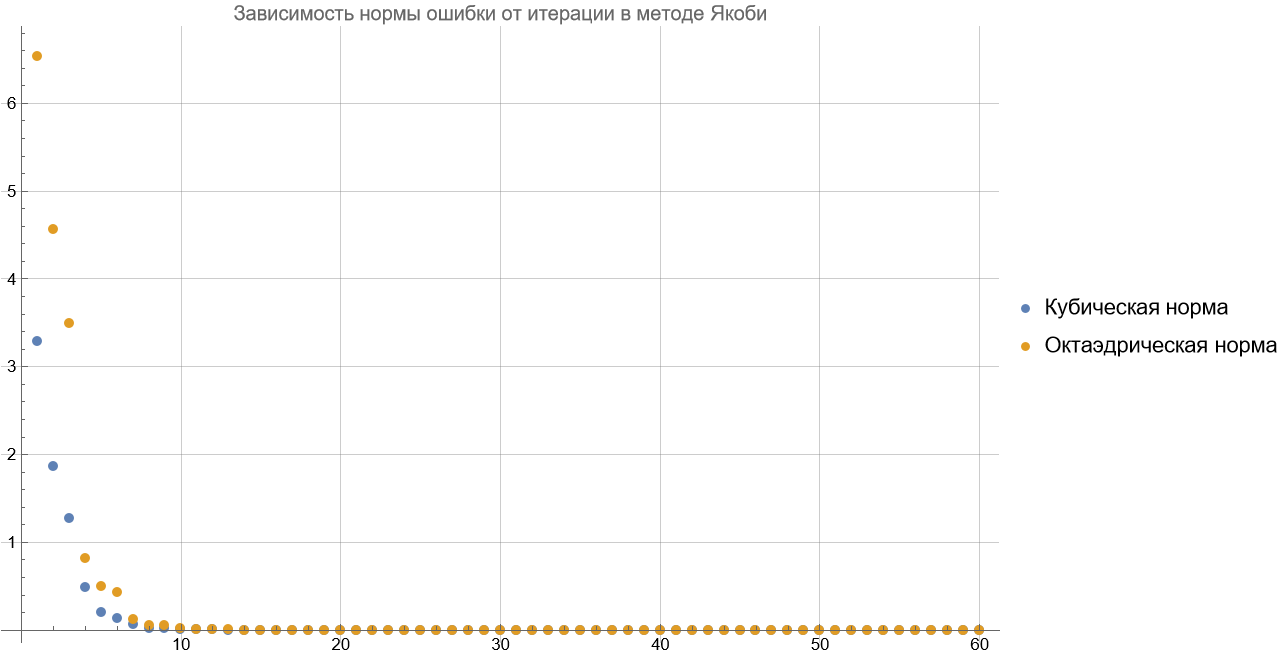
\includegraphics[width=\textwidth]{../lab_iter_methods/graph1_err_vs_iter_jacoby.png}
            \caption{График зависимости нормы ошибкаи от итерации в методе Якоби}
            \label{jacoby_err_vs_iter}
        \end{figure}

        \begin{figure}[H]
            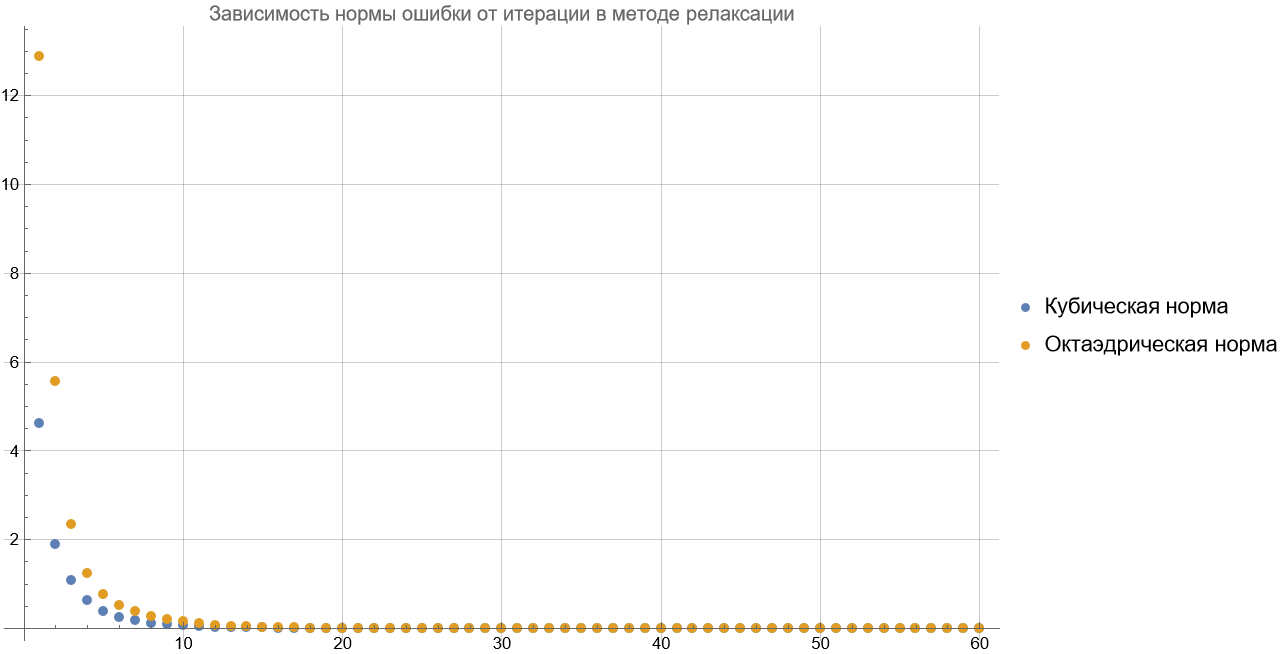
\includegraphics[width=\textwidth]{../lab_iter_methods/graph1_err_vs_iter_relax.png}
            \caption{График зависимости нормы ошибкаи от итерации в методе релаксации}
            \label{relax_err_vs_iter}
        \end{figure}

        \end{enumerate}    
\end{document}
